\chapter*{About Peking University} 
%\addchap{About Peking University}
\rhead{About PKU}
%\addstarredchapter{About Peking University}
%\chaptermark{About Peking University}
\addcontentsline{toc}{chapter}{About Peking University}\mtcaddchapter
\vspace{-5em}

\section*{General Information}
%\addcontentsline{toc}{section}{General Information} 
Peking University is a comprehensive and national key university. The campus, known as "Yan Yuan"(the garden of Yan), is situated at Haidian District in the western suburb of Beijing, with a total area of 2,743,532 square metres (or 274 hectares). It stands near to the Yuanmingyuan Garden and the Summer Palace.

Peking University is proud of its outstanding faculty, including 53 members of the Chinese Academy of Sciences (CAS), 7 members of the Chinese Academy of Engineering (CAE), and 14 members of the Third World Academy of Sciences (TWAS).

The university has effectively combined research on important scientific subjects with the training of personnel with a high level of specialized knowledge and professional skill as demanded by the country's socialist modernization. It strives not only for improvements in teaching and research work, but also for the promotion of interaction and mutual promotion among various disciplines.  

Thus Peking University has become a center for teaching and research and a university of a new type, embracing diverse branches of learning such as basic and applied sciences, social sciences and the humanities, and sciences of medicine, management, and education. Its aim is to rank among the world's best universities in the future. 

\section*{History}
%\addcontentsline{toc}{section}{History}
Founded in 1898, Peking University was originally known as the Imperial University of Peking. It was the first national university covering comprehensive disciplines in China, and has been a leading institution of higher education in China since its establishment. It also served as the highest administration for education at the beginning of its founding. 


In 1912, the university adopted its present name. At the end of the 20th century, the Chinese government put Peking University at the top of its agenda for promoting higher education, with the aim to build a world-class university in the 21st Century. After merging with Beijing Medical University in 2000, Peking University once again was strengthened in its disciplinary structure. 

Peking University has continually played the essential role of pioneers in the course of China's modernization. The university's traditional emphasis on patriotism, progress, democracy, and science, together with its educational standards of diligence, precision, factualism, and innovation, have been passed down from generation to generation. 

%\vspace{3.25em}
%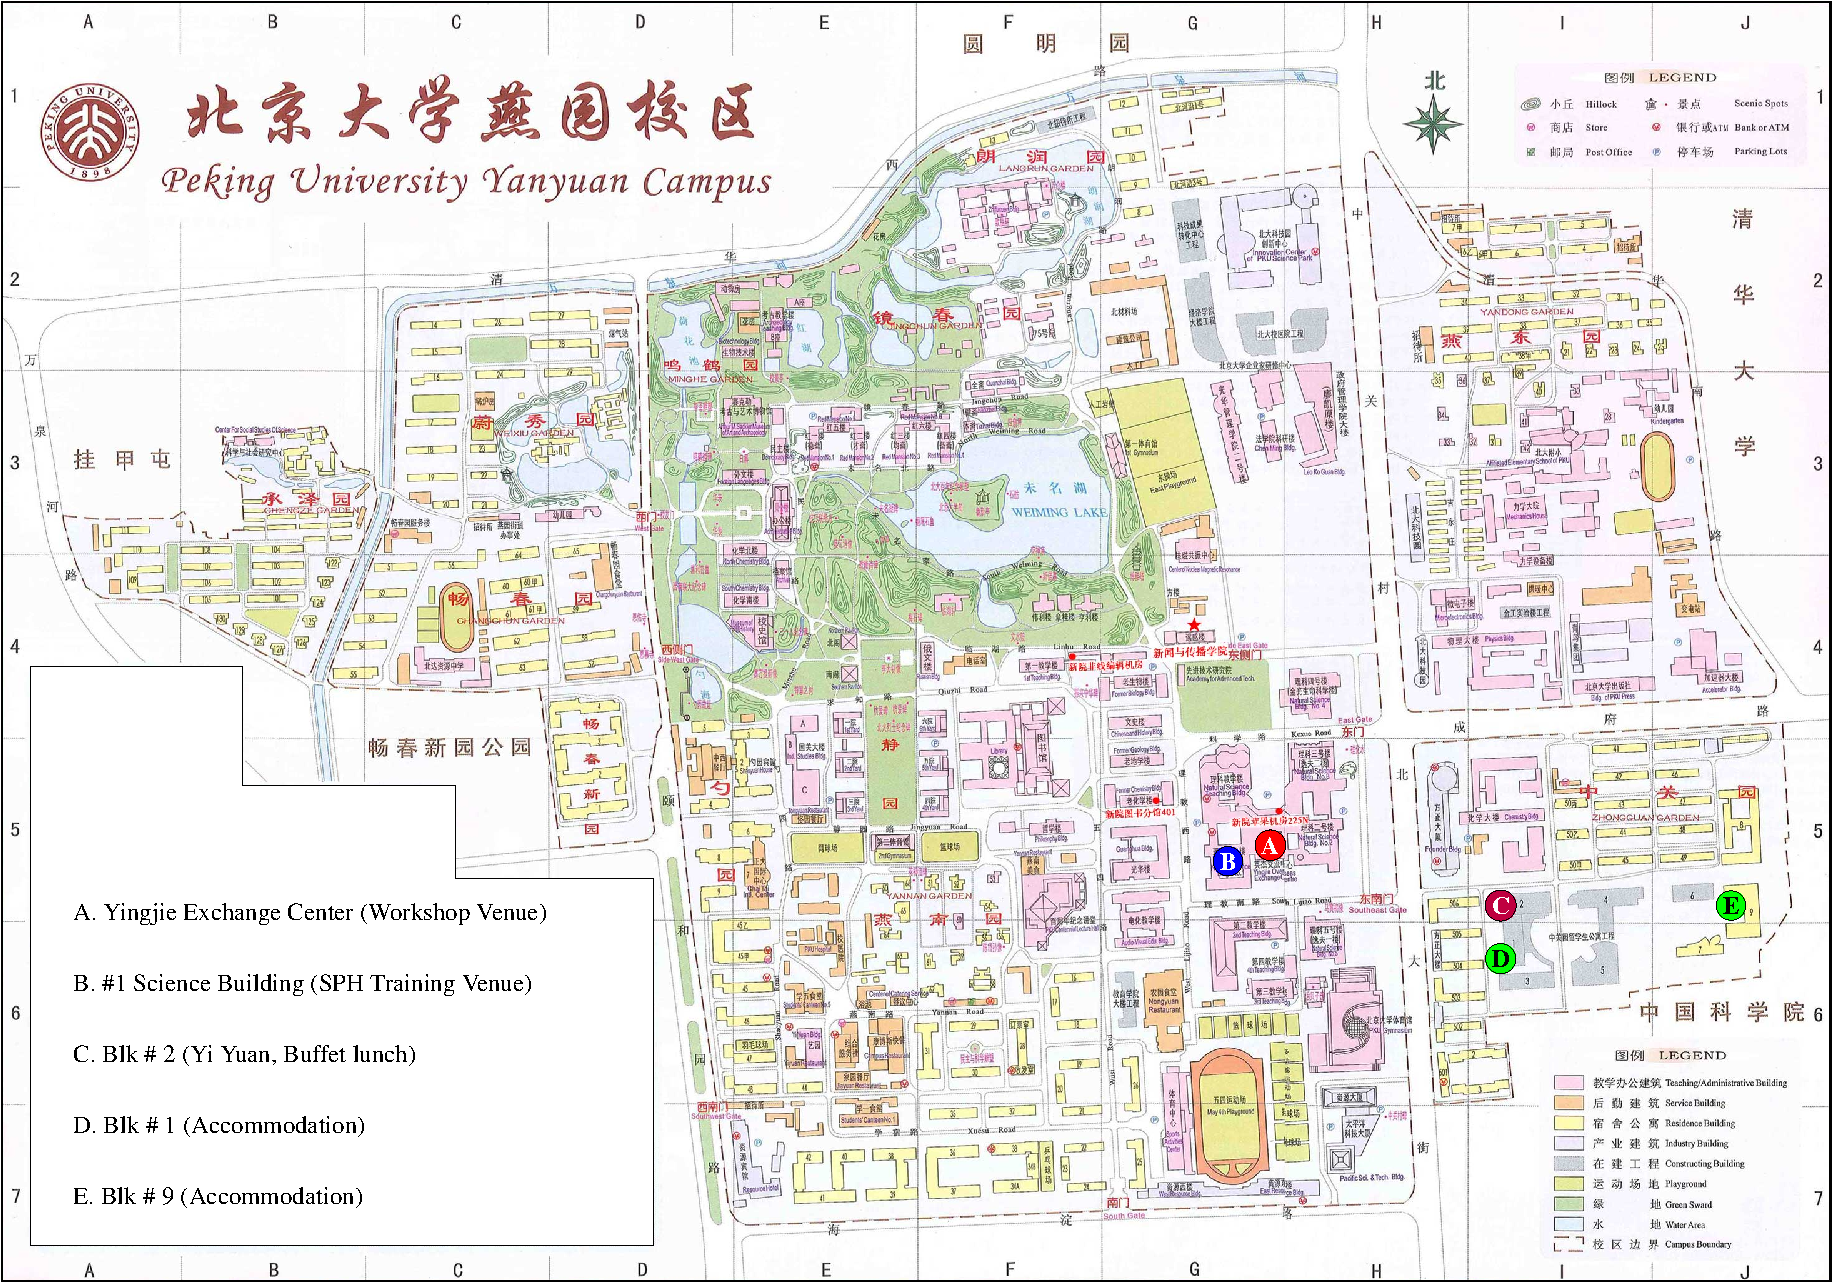
\includegraphics[width=\textwidth]{PKU.jpg}
